\documentclass{article}
\usepackage{amsmath,enumitem,fullpage,graphicx,listings,float,sidecap,setspace,xcolor,wrapfig,booktabs,multirow,subcaption,array,minted,hyperref,xepersian,bidi,svg}
%compile with xelatex+shell+escape
\newcolumntype{C}[1]{>{\centering\arraybackslash}m{#1}}

\definecolor{lg}{HTML}{F4F3F3}
\setlength{\fboxsep}{10pt}
\usemintedstyle{borland}
\hypersetup{
    colorlinks=true,
    linkcolor=blue,
    citecolor=green,
    filecolor=magenta,
    urlcolor=cyan
}
\fontsize{14pt}{16pt}\selectfont
\setlatintextfont{IRNazanin.ttf}
\settextfont{IRNazanin.ttf}

\begin{document}
\begin{titlepage}
    \centering
    \begin{figure}[ht]
        \centering
        
\includegraphics[width=0.5\textwidth]{iust.png}
    \end{figure}
    \vspace{1cm}
    {\scshape\Huge \textbf{دانشکده مهندسی کامپیوتر} \par}
    \vspace{1cm}
    {\huge\bfseries تمرین رادیوم  \par}
    \vspace{1cm}
    {\Large امنیت سیستم‌های کامپیوتری \par}
    \vspace{1cm}
	{\LARGE  مدرس: دکتر ابوالفضل دیانت\par}
    \vspace{1cm}
    {\LARGE  محمدحسین عباسپور، فرزان رحمانی \par}
    \vspace{1cm}
    {\LARGE شماره دانشجویی: ۹۹۵۲۱۴۳۳، ۹۹۵۲۱۲۷۲ \par}
    \vspace{1.22cm}
    {\large نیم سال دوم \par}
    {\large سال تحصیلی ۱۴۰۳-۱۴۰۲ \par}
\end{titlepage}
\newpage
\doublespacing
\singlespacing
\newpage
\setstretch{1.5}
\section*{سوال ۱: امروزه تا چه میزان می‌توان در یک زمان معقول حمله \lr{Brute-force} انجام داد؟ هدف از این سوال این است که بگویید \lr{CPU} یا \lr{GPU}های فعلی تا چه میزان می‌توانند محاسبات را در ثانیه انجام دهند؟ به عنوان نمونه یکی دو مدل به همراه \lr{Becnhmark} آن مثال بزنید.} 
\leavevmode \\

برای شکستن رمز به وسیله الگوریتم \lr{Brute-force} به:
\begin{enumerate}
\item تعداد عملیات مورد نیاز برای شکستن رمز
\item سرعت کامپیوتر و یا به عبارتی \lr{FLOPS}
\end{enumerate}
نیاز داریم. \\
مورد اول به عبارتی بیانگر فضای جستجوی کلید میباشد و مورد دوم هم بیانگر قدرت محاسبه‌گری کامپیوتر در واحد زمان میباشد؛ یا به عبارتی کامپیوتر در یک ثانیه چند عملیات اعشاری را می‌تواند انجام دهد. امروزه کامپیوترهایی با قدرت \lr{10\textsuperscript{18} FLOPS} وجود دارد.
به عنوان مثال ۵ مورد از ابرکامپیوترهای حال موجود در شکل ~\ref{fig1} آورده شده است.
\begin{figure}[h]
\centering
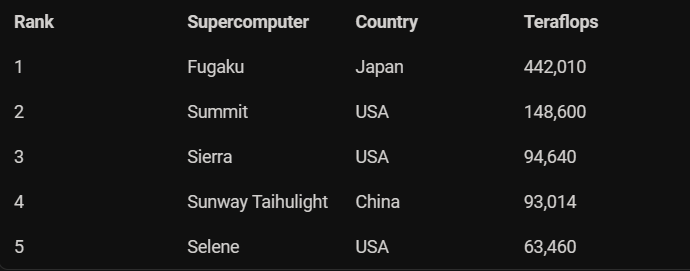
\includegraphics[width=0.5\textwidth]{1.png}
\caption{۵ ابرکامپیوتر برتر دنیا}
\label{fig1}
\end{figure}
برای مثال رمزی که نیاز به \lr{10\textsuperscript{22}} عملیات دارد، در ۱۰۰۰۰ ثانیه توسط کامپیوتر ذکرشده قابل شکستن است. همچنین باید در نظر داشت که رمز در حداکثر چه مدت زمانی باید شکسته شود؛ اگر آن مدت زمان کمتر از ۱۰۰۰۰ ثانیه باشد آنگاه نمیتوان آن را توسط \lr{Brute-force} شکست؛ یا به عبارتی رمز غیرقابل شکستن است.
\begin{itemize}
\item البته کامپیوترهای کوانتومی بسیار سریع‌تر هستند ولی به همان اندازه هم گرون قیمت‌تر میباشند.
\end{itemize}
\newpage
\section*{سوال ۲: آلمان‌ها در طول جنگ جهانی اول از یک سامانه رمزگذاری به نام \lr{Double Transposition} استفاده می‌کردند. در مورد این الگوریتم تحقیق کنید و به طور مختصر آن را توضیح دهید.}
\leavevmode \\
الگوریتم رمزگذاری \lr{Double Transposition} یکی از رمزهای دستی بسیار ایمنی بود که در جنگ جهانی استفاده میشد. این الگوریتم توسط هر دو طرف متحدان و محور به کار گرفته میشد و به خوبی عمل می‌کرد. اما نقطه ضعف اصلی آن این بود که اگر حمله‌کننده دو با بیشتر پیام‌هایی با همان طول و با استفاده از همان کلید را از دسترس برد، می‌توانست با یک فرآیند خسته‌کننده به نام ''آناگرام‌گیری چندگانه'' راه‌حال‌هایی برای هر دو پیام پیدا کند. این ضعف مهم نبود اگر فقط یک پیام با هر کلید ارسال میشد. همچنین، اجرای صحییح این الگوریتم نیاز به دقت زیاد داشت و اگر در نقطه‌ای حساس خطا اتفاق می‌افتاد، رمزگشایی دشوار میشد. در ایالات متحده، اطلاعات مربوط به \lr{CryptoAnalyse} این رمز تا چند سال پیش محرمانه بود. الگوریتم دوگانه تبدیل از دوبار استفاده از تبدیل ستونی برای یک پیام تشکیل شده است. این دو بار ممکن است از همان کلید برای هر دو مرحله استفاده کنند یا ممکن است از کلیدهای متفاوتی استفاده کنند. حال به عنوان مثال میخواهیم متن ''attackxatxdawn'' را رمزگذاری کنیم: (x بیانگر فاصله بین کلمات میباشد)
\begin{enumerate}
\item ابتدا یک جدول اولیه با ابعاد مشخص درست میکنیم؛ سپس حروف متن را به ترتیب داخل جدول قرار میدهیم:
\begin{figure}[h]
\centering
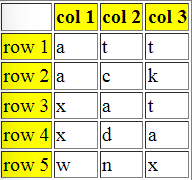
\includegraphics{2.png}
\caption{مرحل اول \lr{Double Transposition}}
\label{fig2}
\end{figure}

\item در مرحله بعد یک جایگشت از ستون‌ها و یک جایگشت از ردیف‌ها را انتخاب میکنیم. به عنوان مثال برای:\\ ستون‌ها (۲, ۳, ۱) و برای ردیف‌ها (۲, ۴, ۱, ۵, ۳)
\begin{figure}[h]
\centering
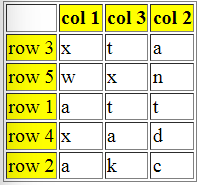
\includegraphics{3.png}
\caption{مرحله دوم \lr{Double Transposition}}
\label{fig3}
\end{figure}
\item در مرحله آخر حروف را به ترتیب کنار هم مینویسیم. متن رمزگذاری شده برابر است با:\\
\lr{xtawxnattxadakc}
\end{enumerate}
\newpage
\section*{سوال ۳}
\leavevmode \\
با استفاده از تحلیل فرکانسی تک حرف‌ها و دو حرف‌ها را میشماریم:\\
\begin{figure}[h]
\centering
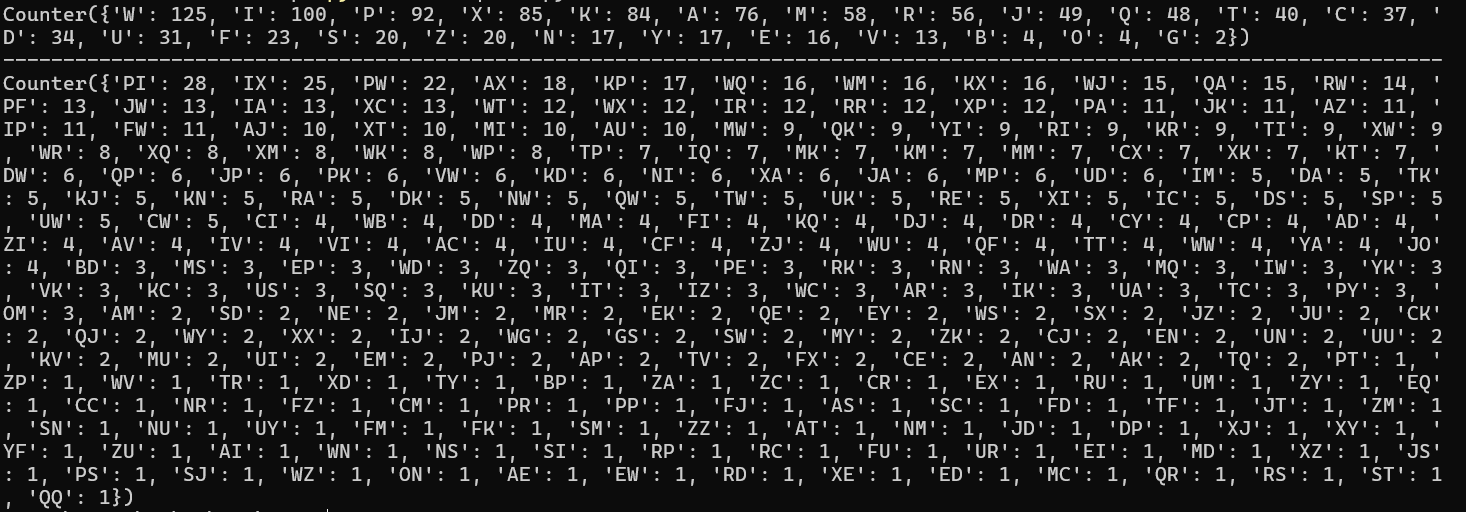
\includegraphics[width=1.0\textwidth]{4.png}
\caption{تحلیل فرکانسی متن}
\end{figure}

حال با استفاده از جداول ~\ref{fig5} و ~\ref{fig6} پر تکرارترین حروف و بایگرام‌های داخل متن را به ترتیب با پر تکرارترین حروف و بایگرام‌های در انگلیسی جایگزین میکنیم و تست میکنیم که آیا متن معنادار میشود یا خیر. به عنوان مثال حرف w که پر تکرارترین متن میباشد با حرف e جایگزین میشود. و به همین ترتیب.\\
\begin{figure}[h]
\centering
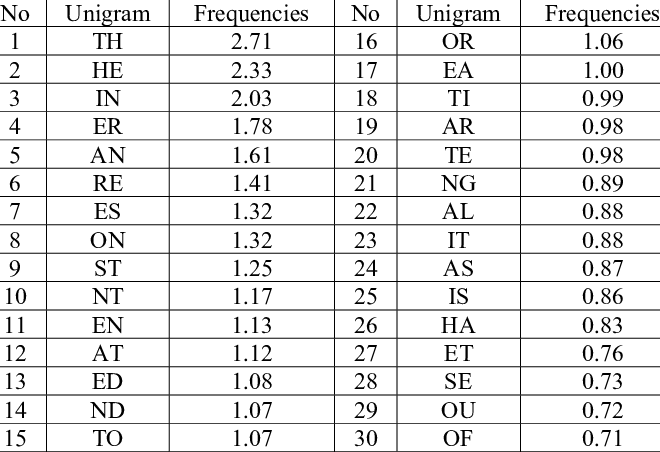
\includegraphics[width=0.7\textwidth]{6.png}
\caption{پر تکرار ترین بایگرام های انگلیسی}
\label{fig6}
\end{figure}
\newpage
\begin{figure}[ht]
\centering
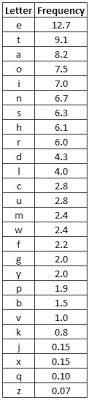
\includegraphics{5.png}
\caption{پر تکرار ترین حروف انگلیسی}
\label{fig5}
\end{figure}

متن اصلی پس از رمزگذاری به شکل زیر خواهد بود:
\begin{figure}[h]
\centering
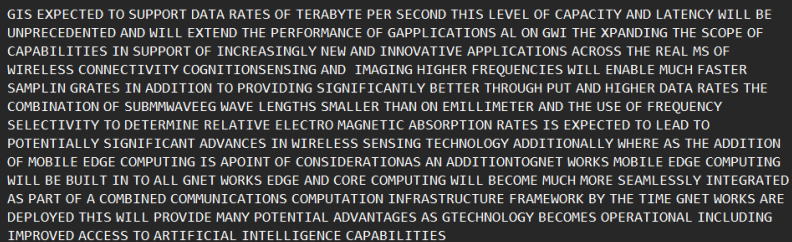
\includegraphics{7.png}
\caption{متن اصلی پس از رمزگشایی}
\end{figure}

\end{document}
